\chapter{Teknologi}
I dette afsnit undersøges Ultralyds Robotarmen ud fra et teknologisk perspektiv. Afsnittet er baseret på besøg hos Hospitalsenheden Horsens og Hospitalsenhed Midt i Viborg. Den teknologiske løsning består af:
\begin{itemize}
\item UR3 Robotarm fra Universal Robots incl. software til styring af denne
\item Stativ til robotten
\item Joystick
\item Computer
\item Holder til ultralydsprobe
\end{itemize}
Denne løsning skal kobles til det allerede eksisterende udstyr. Derfor er produktet en add-on løsning, hvilket betyder at produktet skal købes udover det almindelige scanningsudstyr. Det nuværende system består af Voluson S6 inkl. DICOM og printer, samt diverse ultralydsprober.  

%Se bilag økonomi. 
\begin{figure}[H]
	\begin{minipage}{0.45\textwidth}
		\centering
		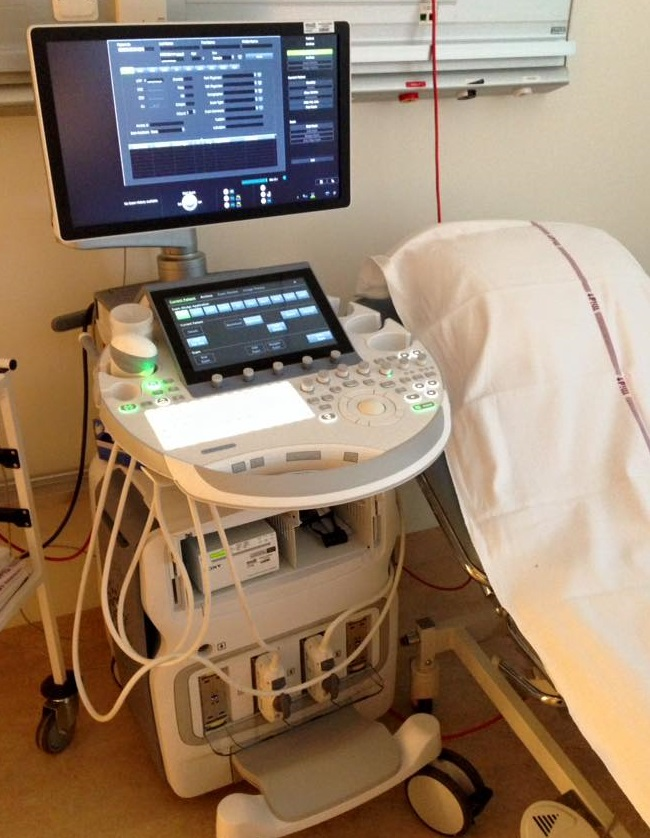
\includegraphics[width=\textwidth]{Figurer/udstyrHorsens.jpg}
		\caption{Nuværende udstyr: Voluson S6 med tilbehør. Billede fra Hospitalsenhed Horsens.}
		\label{udstyrHorsens}
	\end{minipage}
	\hspace{0.02\textwidth}
	\begin{minipage}{0.55\textwidth}
		\centering
		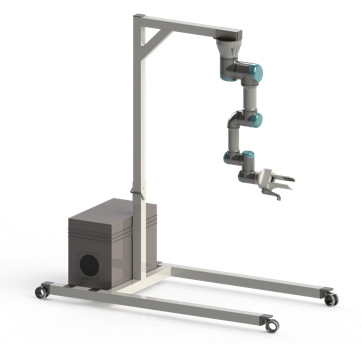
\includegraphics[width=\textwidth]{Figurer/StativMedUR3Render.png}
		\caption{Animation af robotarmen på stativet.}
		\label{Robotstativ}
	\end{minipage}
\end{figure}

\section{Anvendelsesområde}
Produktet skal anvendes til ultralydsscanninger af gravide borgere. Robotarmen er fastmonteret på et stativ, så den hænger over den gravide. Det medvirker en større trykkraft, end hvis den stod på gulvet. For at skabe mobilitet, er stativet placeret på hjul. Hjulene kan låses for af sikkerhedsmæssige årsager og for en statisk placering i forhold til den gravide. På robotarmen findes en universalholder til ultralydsproben. Holderen er universal og passer til alle større fabrikanters håndholdte ultralydsprober, bortset fra vagnialprober.\\

Stativet med robotarmen skal være på den modsatte side af sengen, end sonografen. Dette sikre sonografens udsyn og nærkontakt til den gravide.
Robotarmen skal holde ultralydsproben over den gravide, mens robotarmen styres af sonografen via et joystick. Derved undgår sonografen fysisk akavede arbejdsstillinger. \\
Systemet skal kunne overføre det tryk som sonografen påvirker joysticket med til robotarmen og videre til proben.
Hvis sonografen påvirker joysticket med en kræft større end 15 N, (skal lige tjekkes med Søren) slår robotarmen automatisk fra, af sikkerhedsmæssige grunde. 

\begin{figure}[H]\centering
	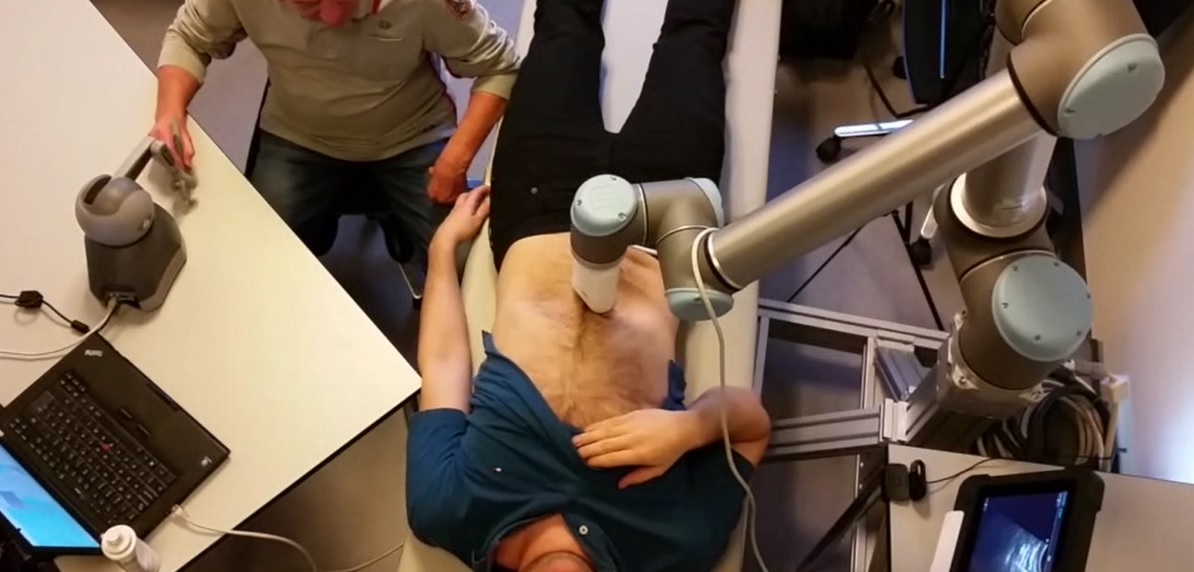
\includegraphics[width = 1.0\textwidth]{Figurer/ergonomiskLosning.jpg}
	\caption{Eksempel på opstilling af Ultralyds Robotarm. Ændringen er at nu vil robotarmen være placeret over borgeren og ikke ved side af. }
	\label{ergonomiskLosning}
\end{figure}

Ultralyds Robotarmen vil blive benyttet til 70-80\% af scannningerne på de gravide, da de sidste 20-30\% af scanningerne er for komplicerede til at robotten kan udføre dem. Derfor skal sonografen manuelt foretage de sidste 20-30\% af scanningerne på den nuværende metode. De komplicerede ultralydsscanninger er blandt andet scanninger på kvinder med højt BMI eller kvinder med bagoverbøjet livmoder. 
\section{Effektivitet}
BMI-problem
Ændrer ikke på produktet - altså samme scanning (der bruges de samme prober)
Tryk - hvordan registreres dette.
\section{Risikovurdering}
pålidelighed
før vs. nu
forbedring af arbejdsstillinger
\section{Delkonklusion}
Ultralyds robotarmen kommer kun til at udføre 70-80\% af scanningerne, hvilket gør at sonograferne stadig skal udføre nogle af scanningerne manuelt. Men at robotarmen kan udføre størstedelen af scanningerne gør, at en stor del af belastningen på sonograferne fjernes. Derfor kan de mest komplicerede scanninger udføres manuelt, da sonograferne vil have mere styrke til disse.

% Kommer sonograferne ud af "træning" - mister styrke??